\documentclass[12pt, varwidth, border={5mm 5mm 5mm 5mm}]{standalone}
\usepackage{tikz}
\usepackage{amsmath}
% Underlining package
\usepackage{ulem}
\usetikzlibrary{angles,quotes}
\usetikzlibrary{intersections}
\usetikzlibrary{arrows.meta}
\usetikzlibrary{calc}
% \usepackage[a4paper, portrait, margin=1cm]{geometry}


\begin{document}
\section*{ }
    
\text{d} = \text{119}^\circ
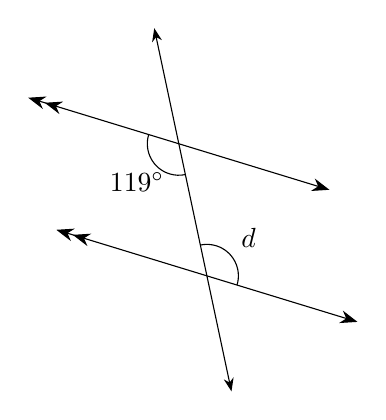
\begin{tikzpicture}[scale=1.0, baseline=(current bounding box.north)]
  \begin{scope}[rotate=102]
    % Draw the first line
    \draw[<->>, >={Stealth[scale=1.3]}, name path=P1] (0, 0) -- (1.9392384809853485, 3.498478828557583);
    % Draw the second line with the calculated offsets
    \draw[<->>, >={Stealth[scale=1.3]}, name path=P2] (1.7150311018099802, 0) -- (3.6542695827953287, 3.498478828557583);
    % Draw the transversal through the middle of the parallel lines
    \draw[<->, >=Stealth, name path=P3] (-0.530380759507326, 1.7492394142787915) -- (4.184650342302655, 1.7492394142787915);
    \path [name intersections={of=P1 and P3,by=A}];
    \path [name intersections={of=P2 and P3,by=B}];
    % Draw the angle
    \coordinate (p1s) at (0, 0);
    \coordinate (p1e) at (1.9392384809853485, 3.498478828557583);
    \coordinate (p2s) at (1.7150311018099802, 0);
    \coordinate (p2e) at (3.6542695827953287, 3.498478828557583);
    \coordinate (ts) at (-0.530380759507326, 1.7492394142787915);
    \coordinate (te) at (4.184650342302655, 1.7492394142787915);
    \draw pic["$d$", draw=black, -, angle eccentricity=1.8, angle radius=0.4cm] {angle=p1s--A--te};
\draw pic["$119^\circ$", draw=black, -, angle eccentricity=1.8, angle radius=0.4cm] {angle=p2e--B--ts};

  \end{scope}
\end{tikzpicture}

\end{document}
